\documentclass[11pt]{article}
\usepackage{ucs}
\usepackage{graphicx}
\usepackage[utf8x]{inputenc} 
\usepackage[russian]{babel}  

\title{ Техническая книга, ФМЛ №30, команда ПСИ}

\begin{document}
	\maketitle
	\tableofcontents{}
	\newpage
	
	\section{Состав команды}
		\begin{table}[h]
			\begin{tabular}{|l|l|l|l|}
				\hline
				\textit{ФИО}         & Год рождения & Место учебы   & Роль в команде                                   \\ \hline
				Жадковский Александр &  1998            & ФМЛ №30       & Капитан команды                                  \\ \hline
				Лутошкин Роман       &  1998         & Гимназия №642 & Ответственный за техническую книгу, оператор № 1 \\ \hline
				Ильясов Александр    &  1999            & ФМЛ №30       & Оператор №2                                      \\ \hline
				Поникаровский Антон  & 1998         & ФМЛ №30       & Запасной оператор                                \\ \hline
			\end{tabular}
		\end{table}
	\section{Описание робота}
		\subsection{Конструкция}
			\begin{itemize}
				\item Робот должен быть небольшим и мобильным
				\item Конструкция должна быть наиболее простой с максимально легким доступом ко всем узлам конструкции
				\item Робот должен обладать механизмом подъема, способным подниматься на высоту 120 см и выше
				\item По возможности робот должен обладать специальным приспособлением для зацепки корзин и их перемещения
			\end{itemize}
		\subsection{Стратегия}
			Период выступления делится на 2(3) периода: автономный период и основное время, которое состоит из первых 1.5 минут и последних 30 секунд.
			В автономном периоде робот должен:
			\begin{itemize}
				\item В зависимости от расположения, съехать с пандуса или выехать вперед
				\item Сориентироваться согласно ИК-датчику и сбить подпорку корзины
				\item Захватить максимально возможное кол-во шариков(Но не более 5-ти)
			\end{itemize}
			После автономного периода следует управляемый двухминутный период в котором необходимо:
			\begin{itemize}
				\item Выгрузить захваченые в автономном периоде шарики в центр. корзину
				\item Захватить новые шарики 
				\item Повторять такую процедуру до окончания времени
				\item В конце вернуться на зону парковки
			\end{itemize}
		
	\section{Основная часть}
	\subsection{16.09.14}
	\begin{enumerate}
		\item Дата собрания : 16.09.14
		\item Цель:
		\begin{itemize}
			\item Собрать основу робота, а именно колесную базу
			\item Написать простейшую программу для управления роботом
		\end{itemize}			
		\item Реализация :
		\begin{itemize}
			\item Была собрана квадратная конструкция(Рис. 1)
			\item Написана программа для передвижения
		\end{itemize}
		\item Результаты
		\begin{itemize}
			\item Собран четырехколесный робот, способный передвигаться по четырем направлениям
			\item Робот управляется с помощью геймпада
		\end{itemize}
		Получившаяся конструкция:
		\begin{figure} [h]
			\centering
			\begin{minipage}{0.3\linewidth}
				\includegraphics[width=35mm,height=35mm]{1_1_robot}\\ Рисунок 1
			\end{minipage}
			\begin{minipage}{0.3\linewidth}
				\includegraphics[width=35mm,height=35mm]{1_2_robot}\\ Рисунок 2
			\end{minipage}
		\end{figure}
	\end{enumerate}
	\newpage
	
	\subsection{3.10.14}
	\begin{enumerate}
		\item Дата собрания 3.10.14
		\item Цель:
		\begin{itemize}
			\item Укрепить конструкцию робота
			\item Разнести колеса по углам конструкции для увеличения площади колесной базы
			\item Закрепить основные узлы управления робота на конструкции с максимально легким доступом к к ним
			\item Оптимизировать программу, перенести управление передвижением робота с кнопок на джойстик
		\end{itemize}
		\item Результаты:
		\begin{itemize}
			\item Конструкция робота была укреплена, центр тяжести снижен 
			\item Двигатели были закреплены по углам конструкции, одновременно закрепляя ее
			\item На осях был закреплен второй ряд колес определенным образом для лучшего управления(Рисунок 2,3)
		\end{itemize}
		\begin{figure} [h]
			\centering
			\begin{minipage}{0.3\linewidth}
				\includegraphics[width=35mm,height=35mm]{3_1_robot}\\ Рисунок 3
			\end{minipage}
			\begin{minipage}{0.3\linewidth}
				\includegraphics[width=35mm,height=35mm]{3_2_robot}\\ Рисунок 4
			\end{minipage}
			\begin{minipage}{0.3\linewidth}
				\includegraphics[width=35mm,height=35mm]{3_3_robot}\\ Рисунок 5
			\end{minipage}
		\end{figure}
		\item Идеи и планы для следующего занятия:
		\begin{itemize}
			\item Начать строить механизм захвата и подъема шариков. В качесте механизма подъема можно использовать ножничный подъемник, механизм захвата еще обдумывается
		\end{itemize}
	\end{enumerate}
	\newpage
	
	\subsection{13.10.14}
	\begin{enumerate}
		\item Дата собрания : 17.10.14
		\item Цель:
		\begin{itemize}
			\item Реализовать ножничный подъемник, механизм, приводящий его в движение и закрепление на кострукции робота
			\item Написать программу для управления захватом с отдельного геймпада
		\end{itemize}
		\item Результаты:
		\begin{itemize}
			\item Робот был частично разобран из-за недостатка деталей, была собрана примерная схема механизма передвижения подъемника(Рисунок 6)
			\item Написать и отладить программу не получилось, опять же из-за отсутствия деталей
		\end{itemize}
		\item Идеи:
		\begin{itemize}
			\item Заменить текущие рейки в подъемнике на алюминиевые профили для удобства установки, увеличения длины составляющих подъемника и уменьшения веса конструкции
			\item Отказаться от омниколес, поставить 4 обычных колеса
		\end{itemize}
		\item Рисунки:
		\begin{figure} [h]
			\centering
			\begin{minipage}{0.3\linewidth}
				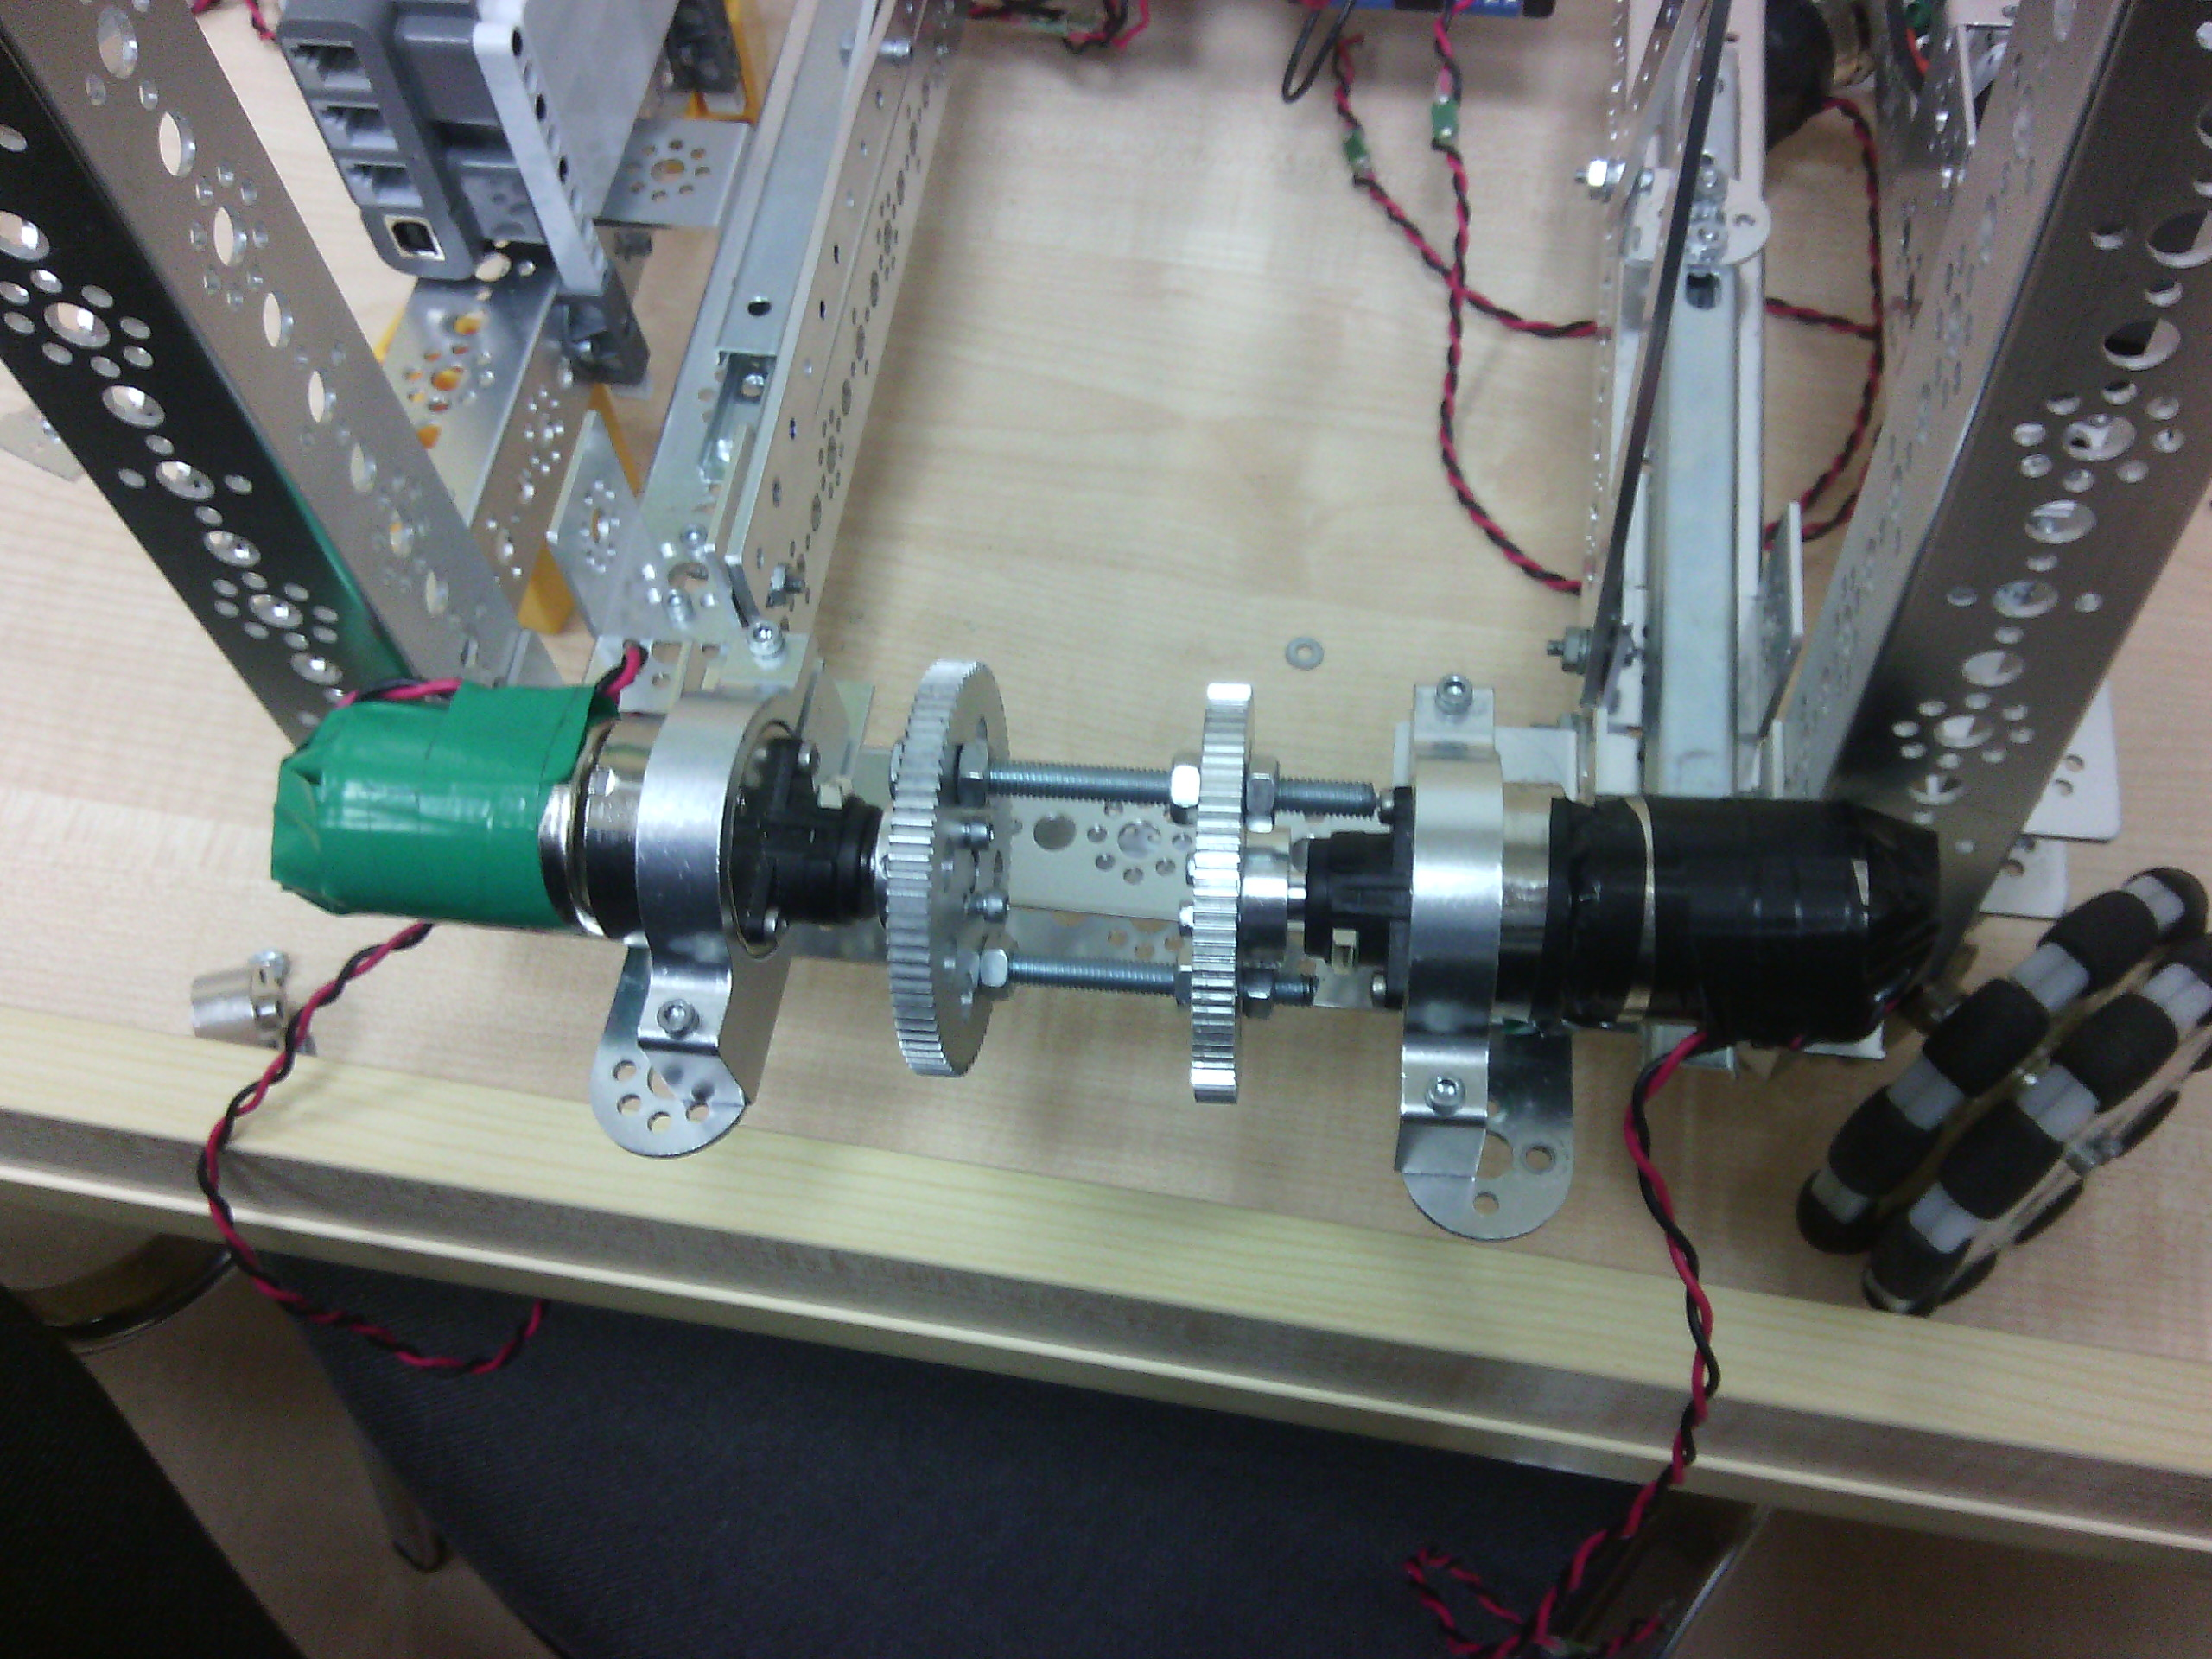
\includegraphics[width=35mm,height=35mm]{5_1_robot}\\ Рисунок 6
			\end{minipage}
			\begin{minipage}{0.3\linewidth}
				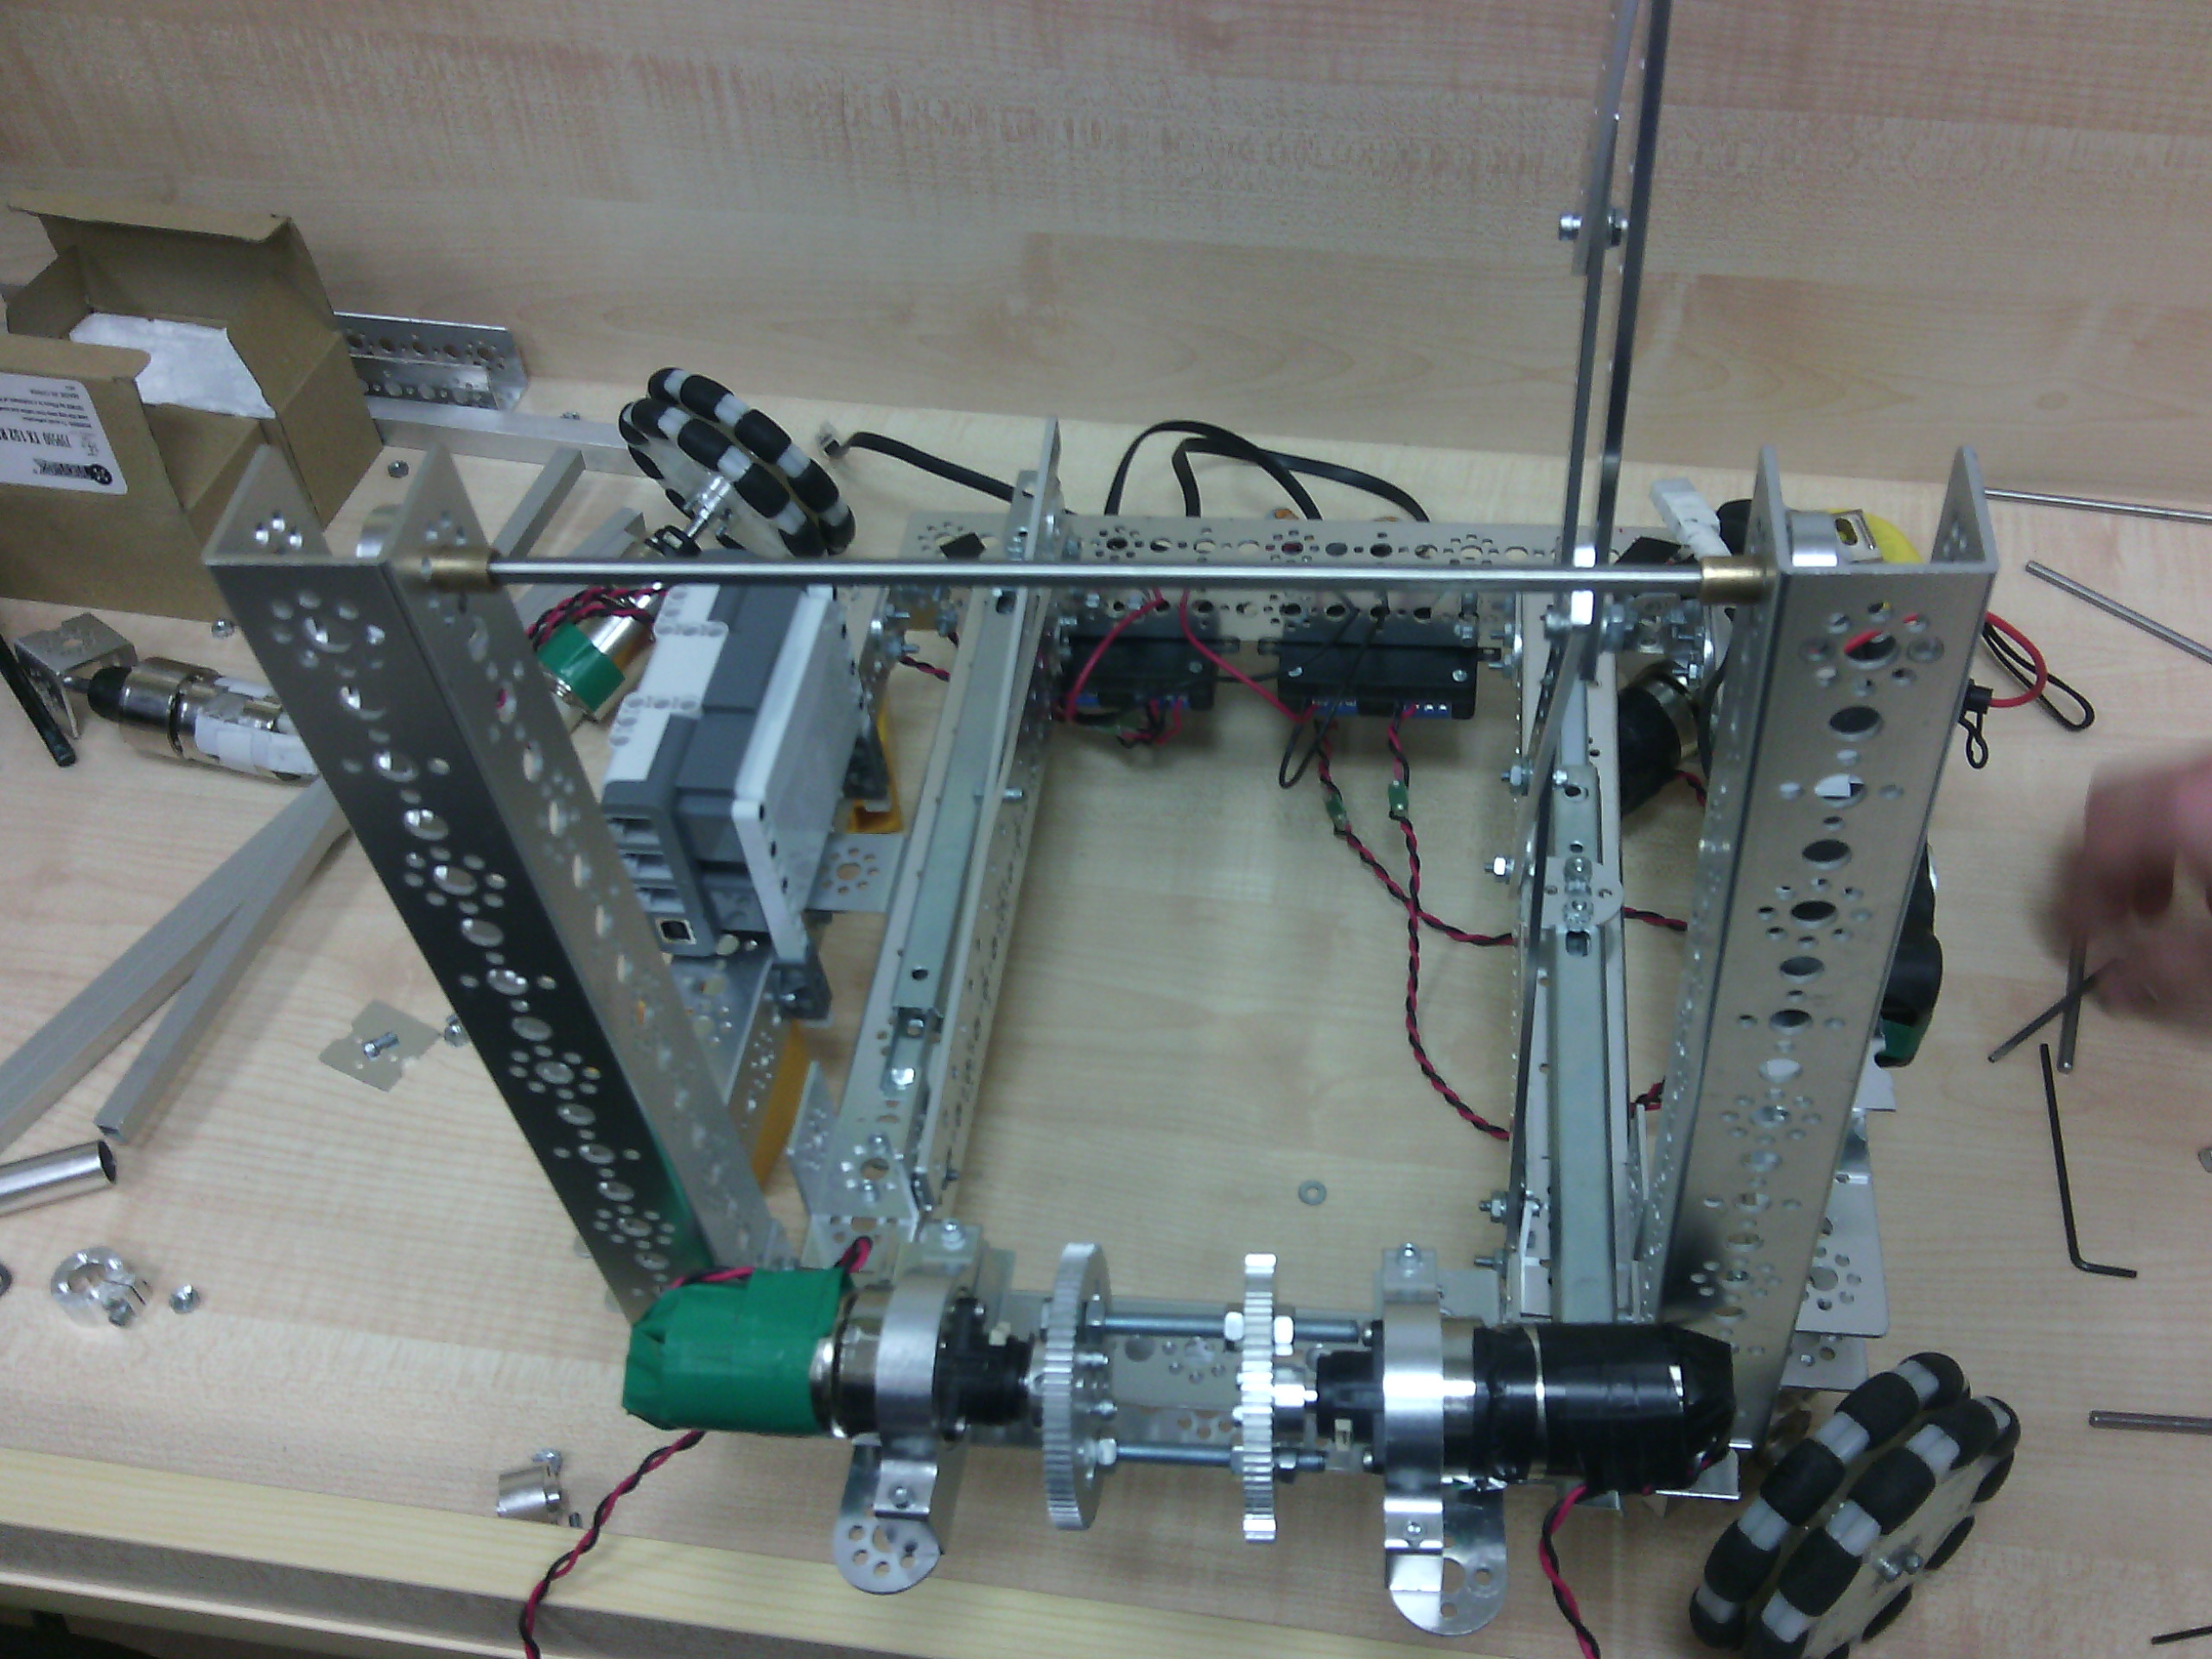
\includegraphics[width=35mm,height=35mm]{5_2_robot}\\ Рисунок 7
			\end{minipage}
		\end{figure}
	\end{enumerate}

	
\end{document}